% taylor-couette.tex

\section{Taylor Couette Flow}
\label{taylor-couette}\index{boundary conditions!MovingWallBC!example of use}
%
This test case, used to verify the nonzero rotational speed version of the Moving-Wall boundary condition,
was provided by Jason Qin. 
It selects some examples of compressible Taylor-Couette flow from Ref.\,\cite{larignon_etal_2006a} 
for an annulus with inner radius 215.5\,mm and gap width 3.1\,mm.
The axial extent of the annulus is 10 times the gap width.
The outer cylindrical surface of the annulus (the housing) was fixed and 
the inner surface (the rotor) was moving with a rotational speed of 27600\,rpm.
Three different pressures are simulated to cover a range of cases, with and without Taylor vortices. 
Other parameters used for the simulations are shown in Table~\ref{ex_data}.

\begin{table}[ht]
  \caption{Parameters for simulations, used match the experimental conditions 
           reported in Ref.\cite{larignon_etal_2006a}}
  \label{ex_data}
  \begin{center}
    \begin{tabular}{lrrr}
     \hline
     \hline
     Case                    & intermediate & high     & low \\ 
                             & pressure     & pressure & pressure \\ \hline
     Pressure, $Pa$          & 100          & 1000     & 10 \\
     Rotor Temperature, $K$  & 348          & 351      & 344 \\
     Stator Temperature, $K$ & 350          & 366      & 344 \\
     Taylor Number           & 17           & 181      & 3.6 \\
     \hline
     \hline
    \end{tabular}
  \end{center}
\end{table}

\bigskip
\subsection{Input script (.py)}
%
To simulate this test case, only a small segment of the annulus is modelled, 
then periodic boundary conditions are applied to connect the ends of the segment.
Note that the ends of the segment have different spatial orientations and this must
be handled by the boundary condition. 
For the low and intermediate pressure cases, since the Taylor numbers are quite low, there is no vortices generated.
In those cases, the grid is low resolution in $z$ direction while, for high pressure case, 
the vortices might be generated in the gap, and it needs a high resolution grid in $z$ direction
(\textit{i.e.} the axial direction of the rotor).

\noindent\topbar
\lstinputlisting[language={}]{../3D/taylor-couette/tc_flow_nitrogen.py}
\bottombar


\subsection{Shell scripts}
\label{tc-sh-files}
\topbar
\lstinputlisting[language={}]{../3D/taylor-couette/prep.sh}
\bottombar

\noindent
\topbar
\lstinputlisting[language={}]{../3D/taylor-couette/tc_flow_nitrogen.sh}
\bottombar

\noindent
\topbar
\lstinputlisting[language={}]{../3D/taylor-couette/post.sh}
\bottombar


\subsection{Results}
%
For the low pressure case, the velocity profile is roughly linear accross the narrow gap, and the temperature
profile has a parabolic shape with maximum temperature near the center of the gap. 
Figure~\ref{tcl-tv-fig} shows the comparison results of velocity and temperature with different methods.
The apparent difference is caused by the slip-wall boundary condition being considered in DSMC method and
a no-slip boundary condition being used by Eilmer3. 
This is not too much of a problem because, with pressure increases, 
the real boundary condition more-closely approaches the no-slip condition.

\begin{figure}[htbp]
\begin{center}
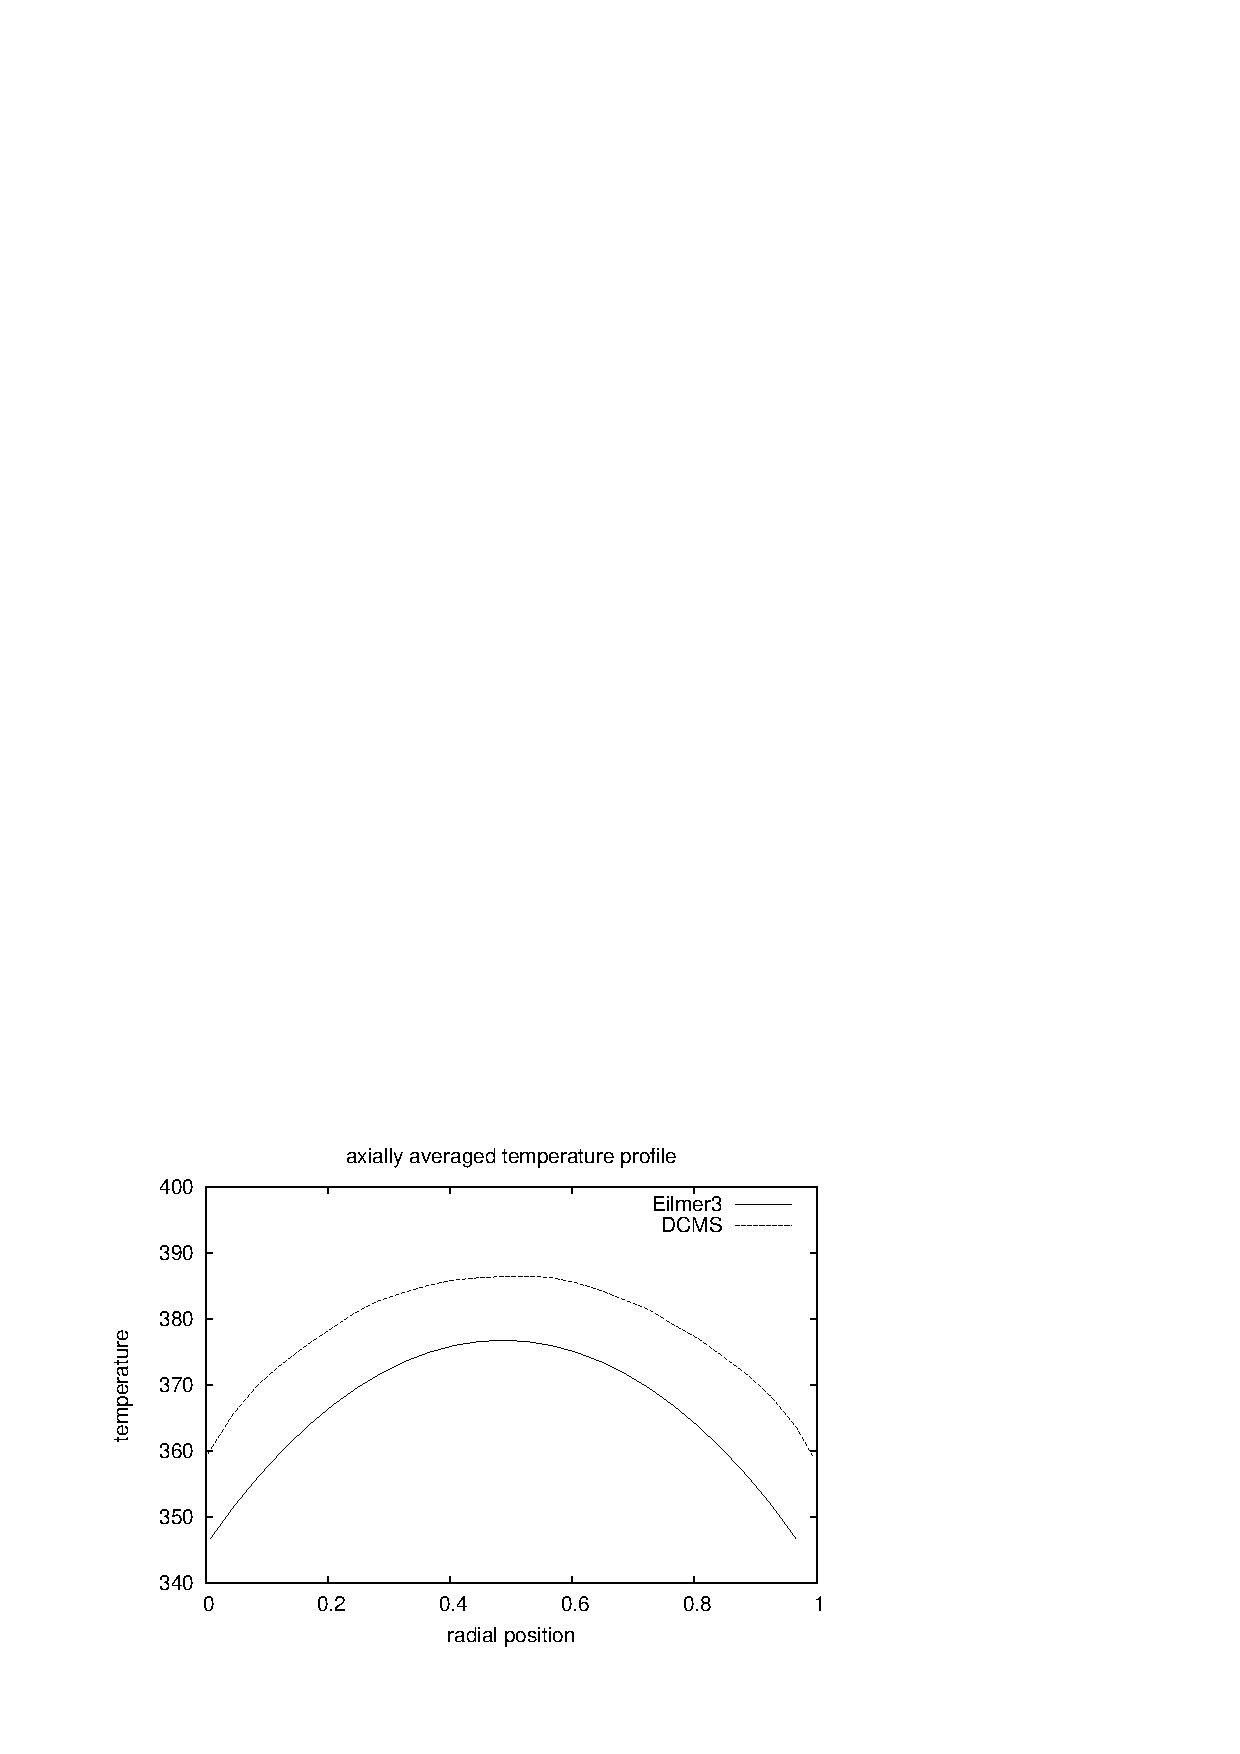
\includegraphics[width=0.45\textwidth,viewport=41 46 411 298,clip=true]{../3D/taylor-couette/temperature-low.pdf}
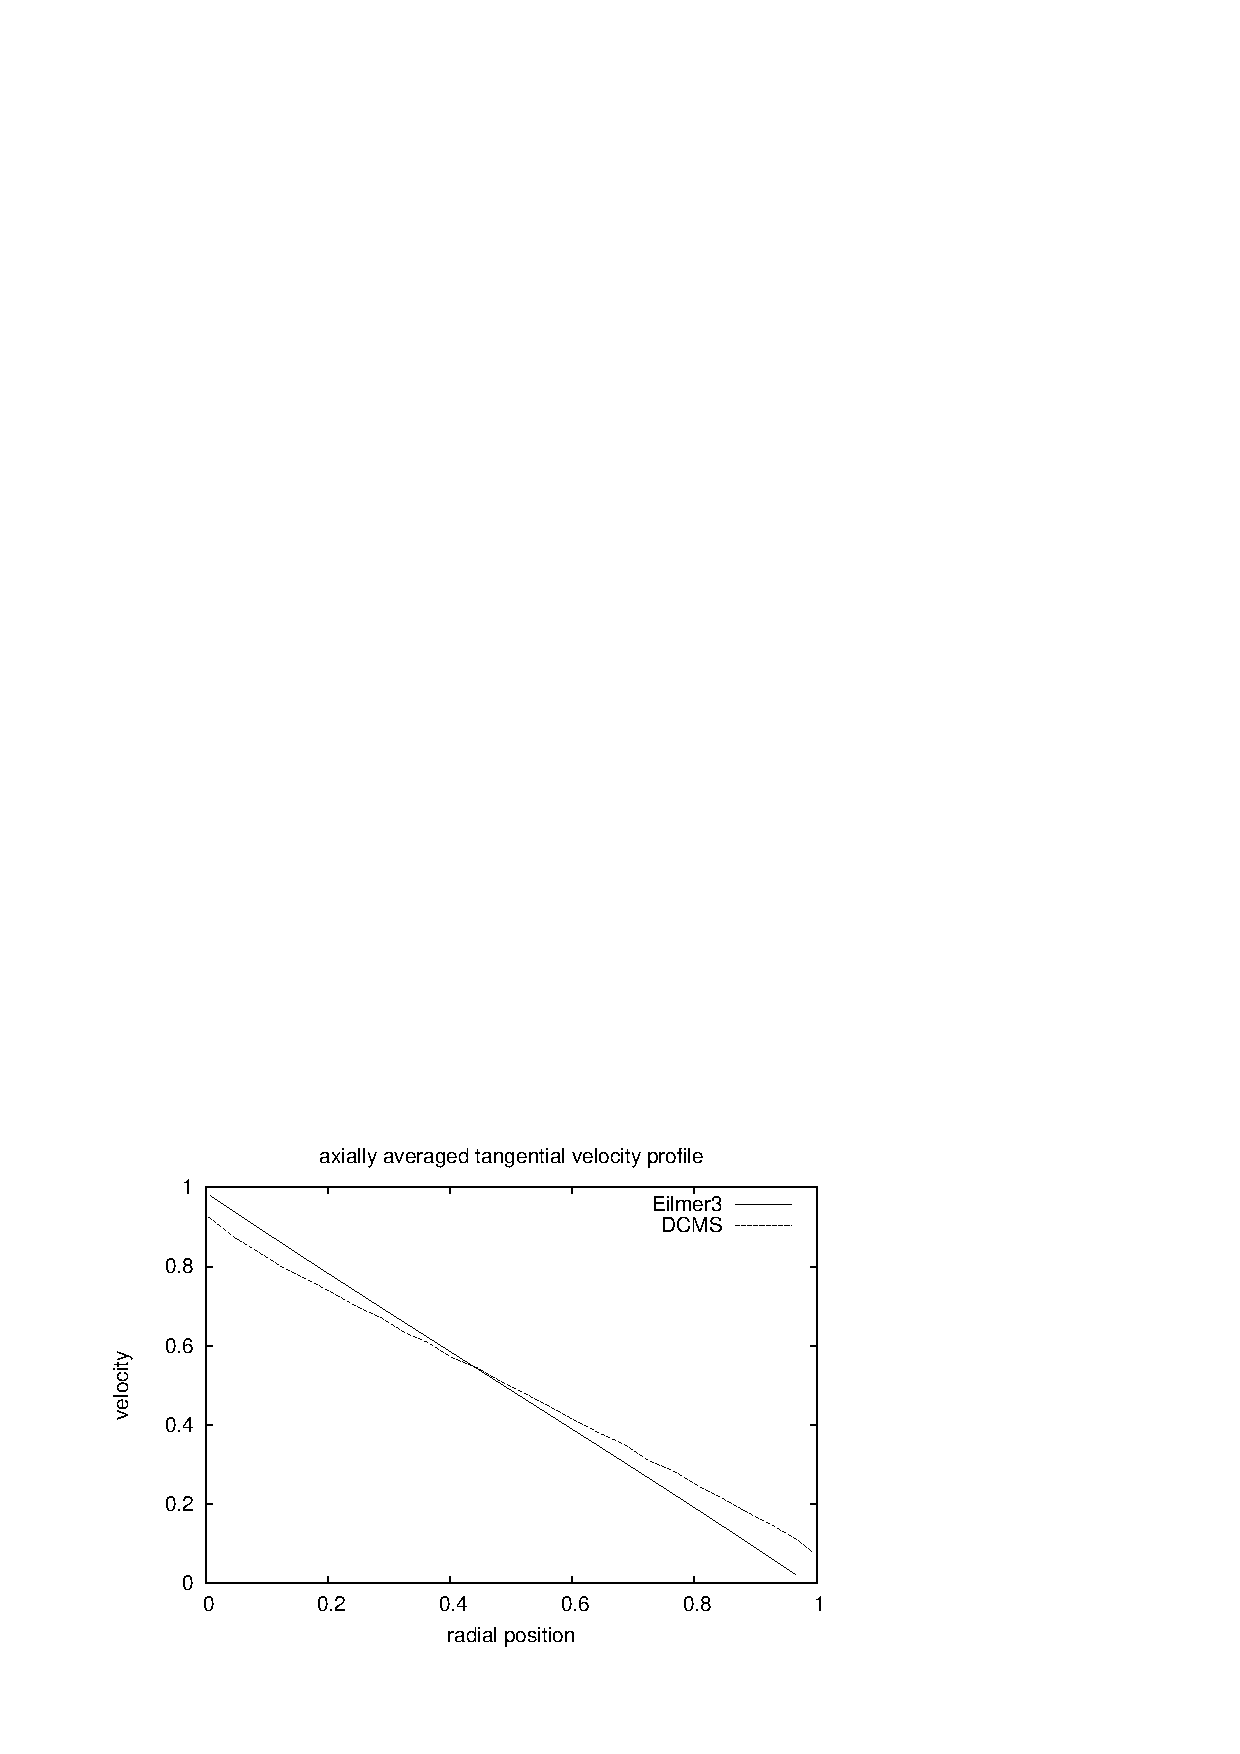
\includegraphics[width=0.45\textwidth,viewport=41 50 407 303,clip=true]{../3D/taylor-couette/velocity-low.pdf}
\end{center}
\caption{Comparison of temperature and velocity profiles in radial direction at low pressure condition.}
\label{tcl-tv-fig}
\end{figure}

\medskip
For the intermediate pressure case, shown in Figure~\ref{tci-tv-fig}, there is a similar result. 
The profile for the tangential velocity is nearly linear
and the temperature profile is nearly parabolic with a maximum slightly closer to the hotter wall as seen in
The agreement between numercial schemes is now good.

\begin{figure}[htbp]
\begin{center}
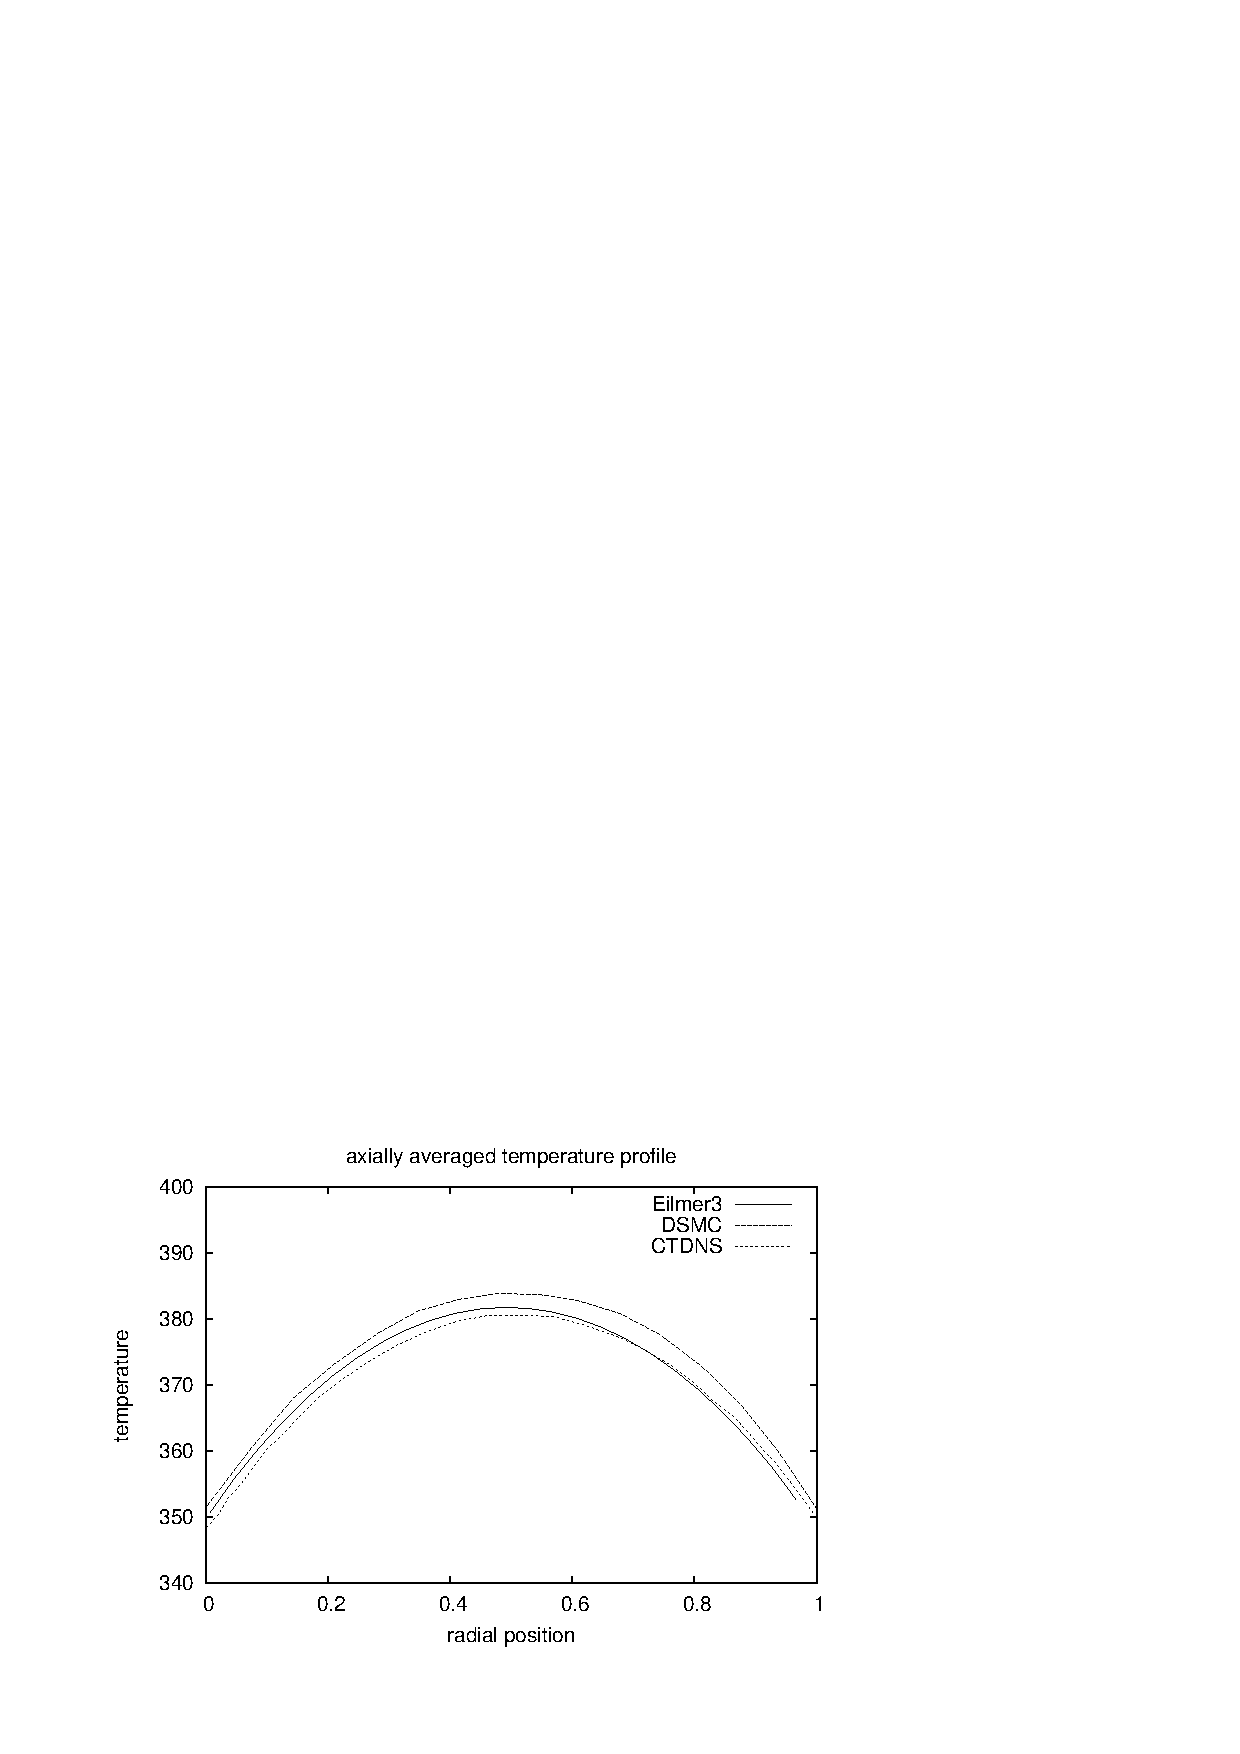
\includegraphics[width=0.45\textwidth,viewport=41 46 411 298,clip=true]{../3D/taylor-couette/temperature-intermediate.pdf}
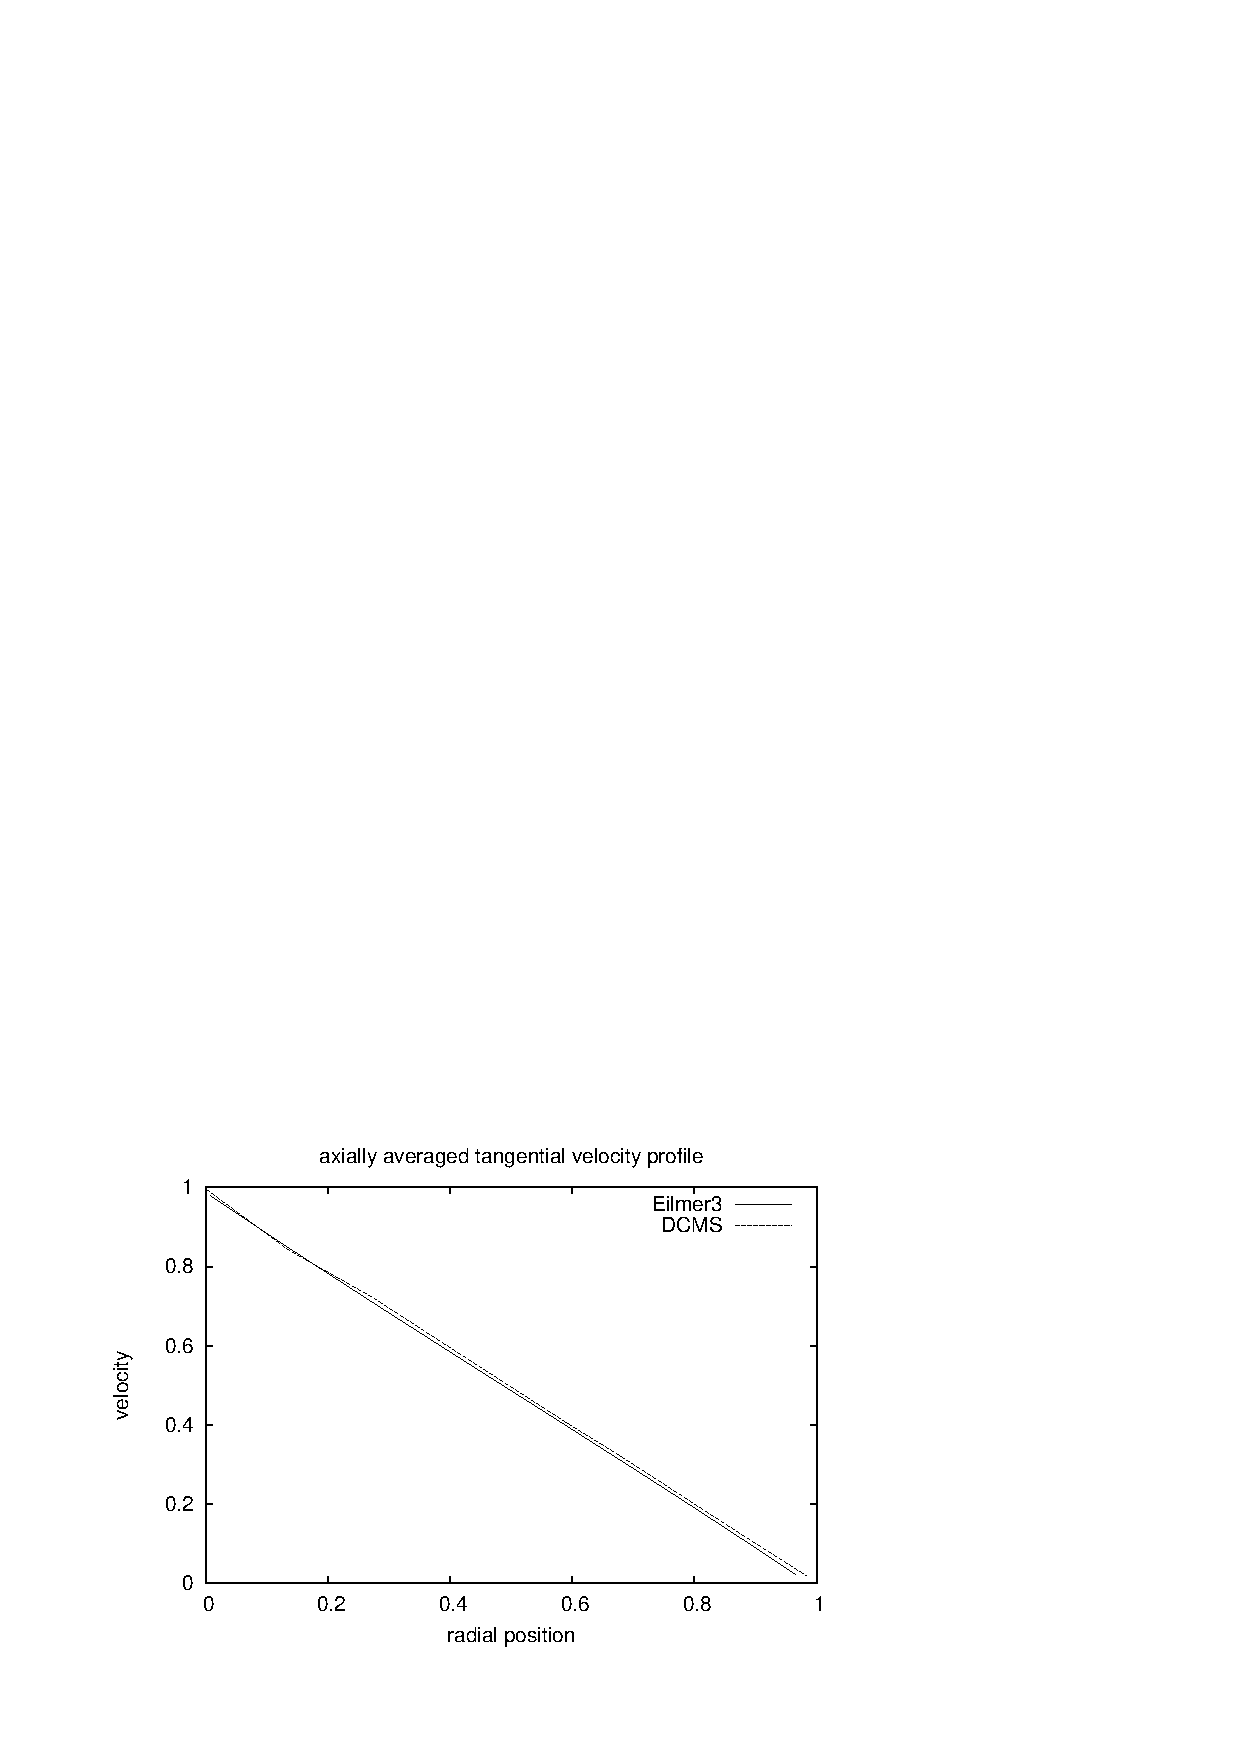
\includegraphics[width=0.45\textwidth,viewport=41 50 407 303,clip=true]{../3D/taylor-couette/velocity-intermediate.pdf}
\end{center}
\caption{Comparison of temperature and velocity profiles in radial direction at intermediate pressure condition.}
\label{tci-tv-fig}
\end{figure}

\medskip
For the high pressure case, the Taylor number has exceeded a critical value and vortices,
aligned with the surface velocity of the rotor, make the gap flow fully three dimensional.
Figure~\ref{tv-fig} shows velocity and temperature contours within the gap, 
the periodic structure being associated with the Taylor vortices.

\begin{figure}[htbp]
\begin{center}
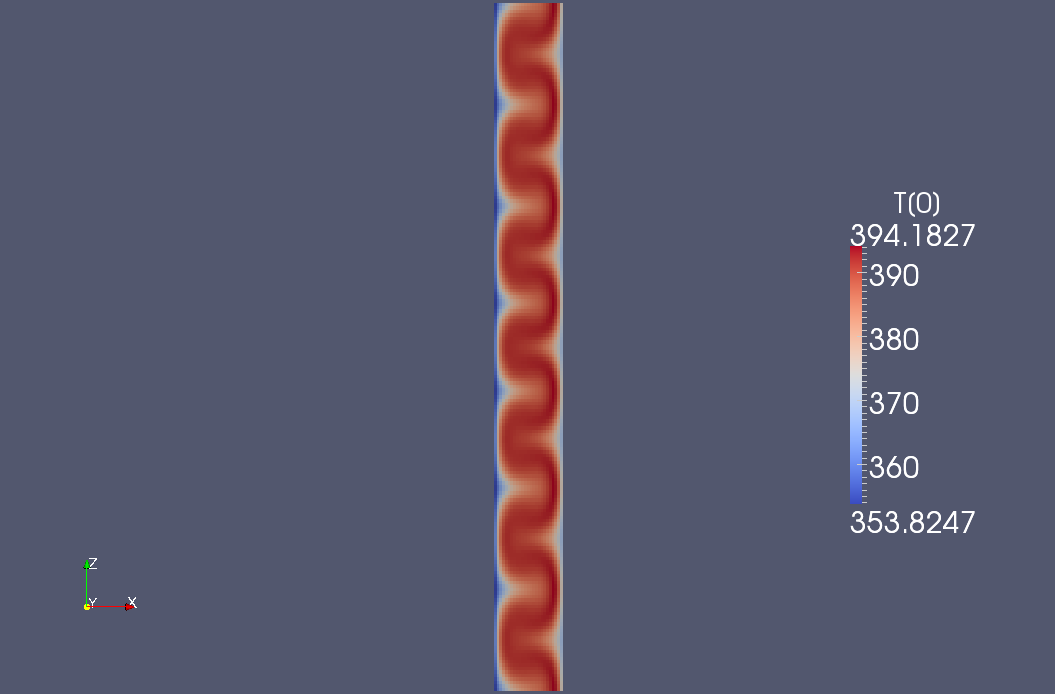
\includegraphics[width=0.45\textwidth]{../3D/taylor-couette/temperature.png}
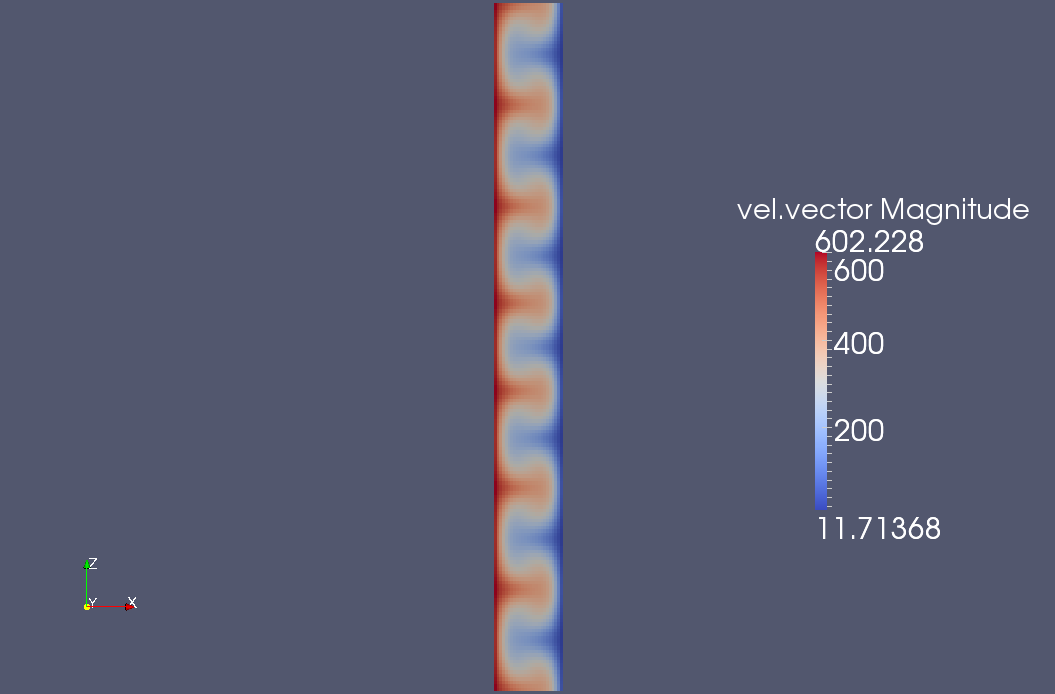
\includegraphics[width=0.45\textwidth]{../3D/taylor-couette/velocity.png}
\end{center}
\caption{Temperature and velocity contours within the gap, at the high pressure condition.
         The left-most boundary is the rotor and the right-most surface is the housing wall.}
\label{tv-fig}
\end{figure}

\medskip
The velocity profile (averaged over the axial direction) has changed to an ``S''-shapes curve 
in Figure~\ref{tch-fig}). 
This velocity profile characterizes a flow with a higher gradient at the walls,
due to enhanced radial transport of fluid induced by the vortices.

\medskip
The axially averaged temperature profile (seen in Figure~\ref{tch-fig}) 
is much flatter than the parabolic profiles of the lower Taylor number cases.
This averaged shape also exhibits steeper graidents at the walls, 
which induce a high heat flux. 
Again, these changes are due to the presence of vortices and the associated increase in radial transport
across the gap.

\begin{figure}[htbp]
\begin{center}
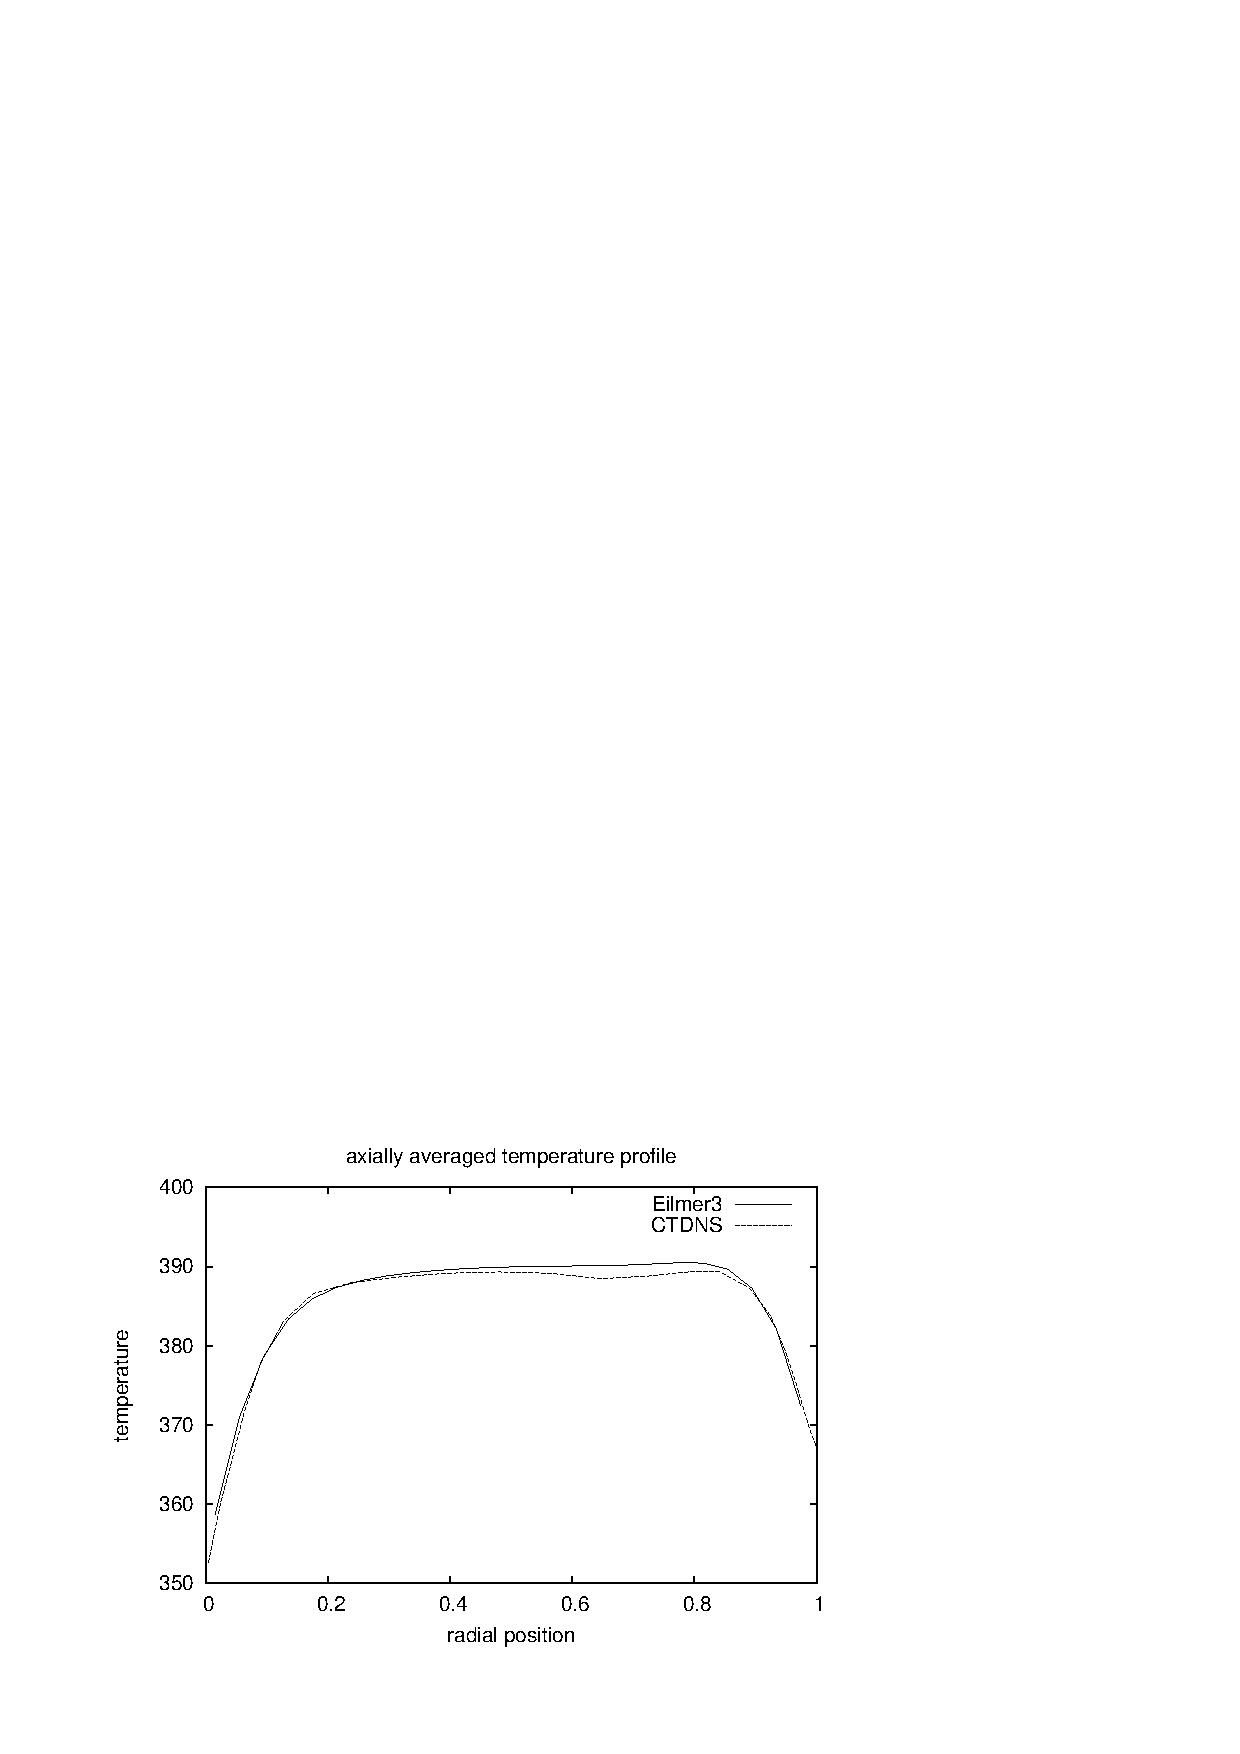
\includegraphics[width=0.45\textwidth,viewport=41 46 411 298,clip=true]{../3D/taylor-couette/temperature-high.pdf}
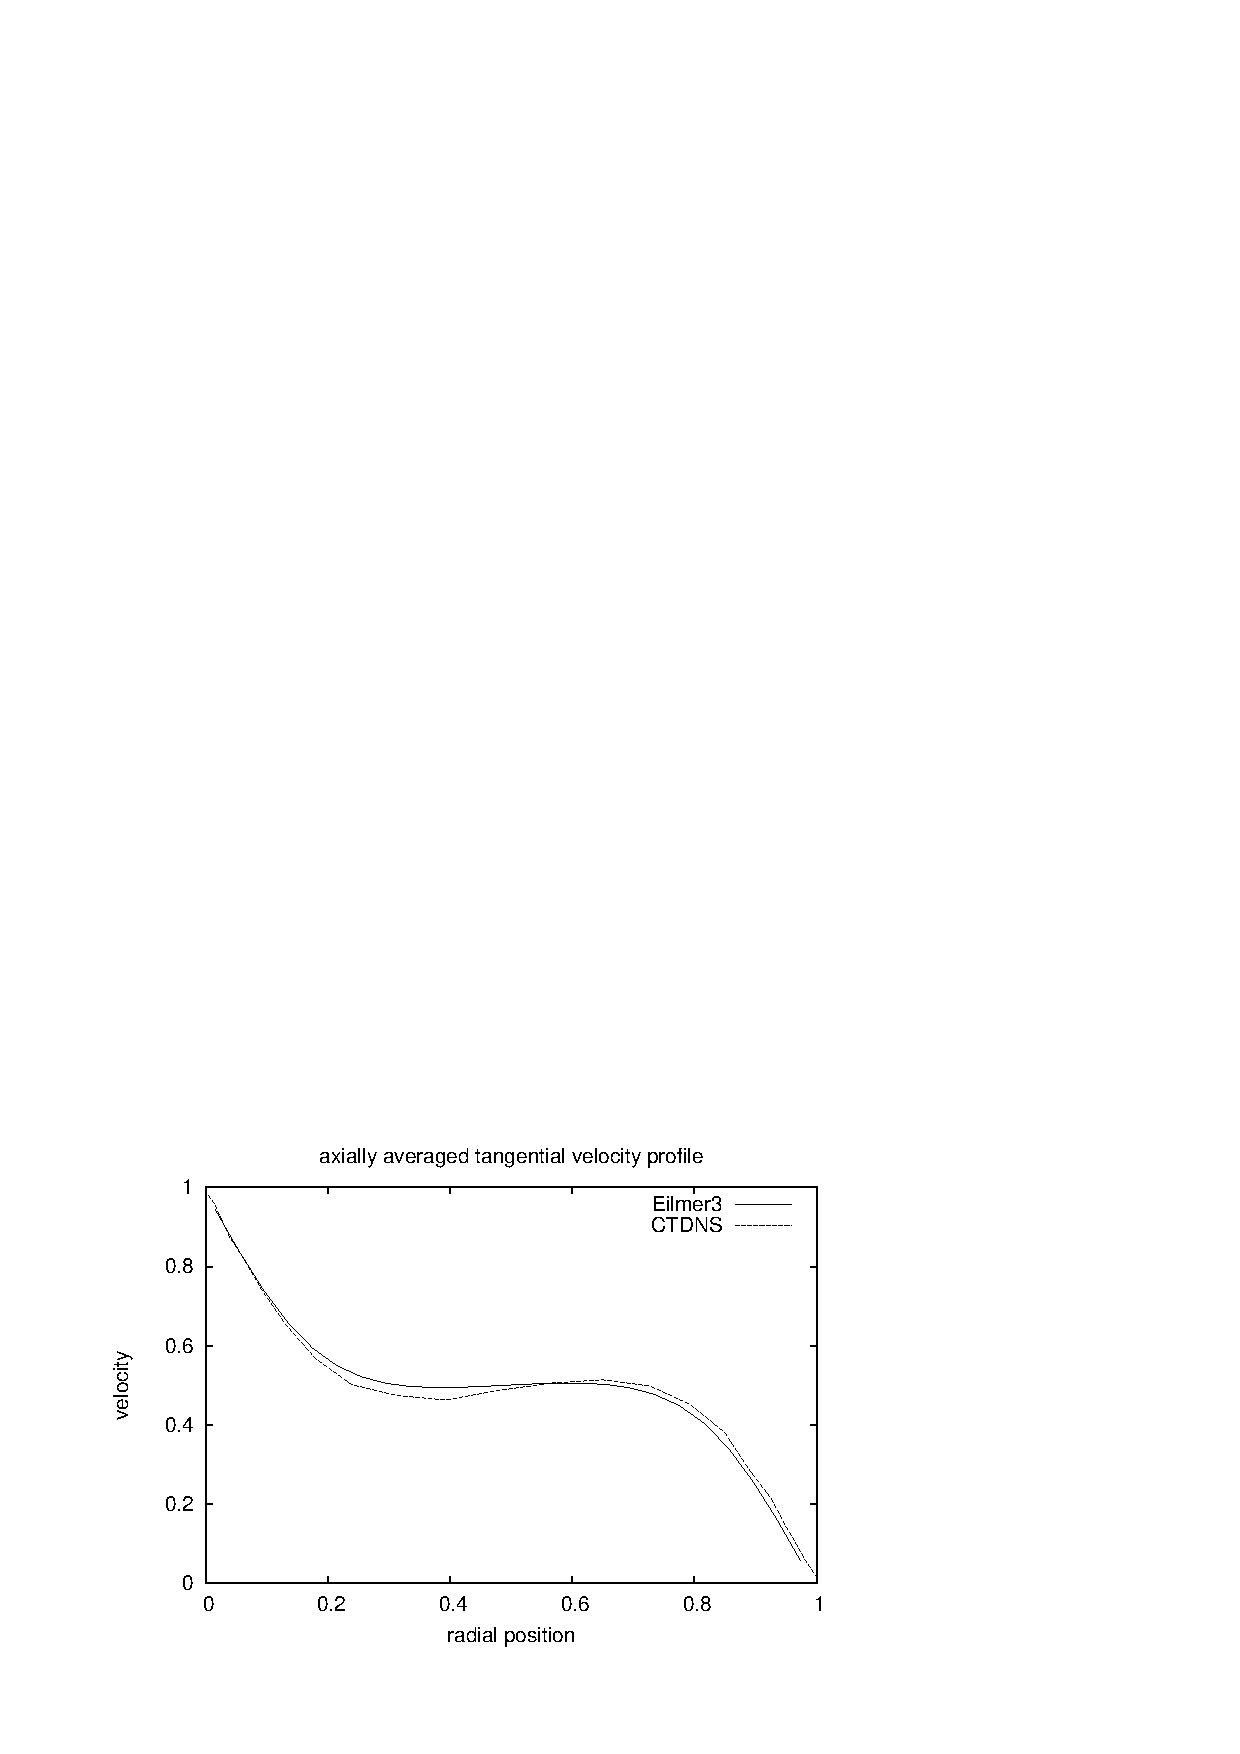
\includegraphics[width=0.45\textwidth,viewport=41 50 407 303,clip=true]{../3D/taylor-couette/velocity-high.pdf}
\end{center}
\caption{Comparison of averaged temperature velocity profiles in radial direction at high pressure condition.}
\label{tch-fig}
\end{figure}


\subsection{Notes}
\begin{itemize}
\item Python script for calculating axially averaged temperature and velocity profile.
      \lstinputlisting[language={}]{../3D/taylor-couette/a_vt.py}
\end{itemize}
